
%%%%%%%%%%%%%%%%%%%%%%%%%%%%%%%%%%%%%%%%%
% Short Sectioned Assignment LaTeX Template Version 1.0 (5/5/12)
% This template has been downloaded from: http://www.LaTeXTemplates.com
% Original author:  Frits Wenneker (http://www.howtotex.com)
% License: CC BY-NC-SA 3.0 (http://creativecommons.org/licenses/by-nc-sa/3.0/)
%%%%%%%%%%%%%%%%%%%%%%%%%%%%%%%%%%%%%%%%%

%----------------------------------------------------------------------------------------
%	PACKAGES AND OTHER DOCUMENT CONFIGURATIONS
%----------------------------------------------------------------------------------------

\documentclass[paper=a4, fontsize=11pt]{scrartcl} % A4 paper and 11pt font size

% ---- Entrada y salida de texto -----

\usepackage[T1]{fontenc} % Use 8-bit encoding that has 256 glyphs
\usepackage[utf8]{inputenc}
%\usepackage{fourier} % Use the Adobe Utopia font for the document - comment this line to return to the LaTeX default

% ---- Idioma --------

\usepackage[spanish, es-tabla]{babel} % Selecciona el español para palabras introducidas automáticamente, p.ej. "septiembre" en la fecha y especifica que se use la palabra Tabla en vez de Cuadro

% ---- Otros paquetes ----

\usepackage{url} % ,href} %para incluir URLs e hipervínculos dentro del texto (aunque hay que instalar href)
\usepackage{amsmath,amsfonts,amsthm} % Math packages
%\usepackage{graphics,graphicx, floatrow} %para incluir imágenes y notas en las imágenes
\usepackage{graphics,graphicx, float} %para incluir imágenes y colocarlas
\usepackage{subfigure} % subfiguras

% Para hacer tablas comlejas
%\usepackage{multirow}
%\usepackage{threeparttable}

%\usepackage{sectsty} % Allows customizing section commands
%\allsectionsfont{\centering \normalfont\scshape} % Make all sections centered, the default font and small caps

\usepackage{fancyhdr} % Custom headers and footers
\usepackage{pdflscape}

\pagestyle{fancyplain} % Makes all pages in the document conform to the custom headers and footers
\fancyhead{} % No page header - if you want one, create it in the same way as the footers below
\fancyfoot[L]{} % Empty left footer
\fancyfoot[C]{} % Empty center footer
\fancyfoot[R]{\thepage} % Page numbering for right footer
\renewcommand{\headrulewidth}{0pt} % Remove header underlines
\renewcommand{\footrulewidth}{0pt} % Remove footer underlines
\setlength{\headheight}{13.6pt} % Customize the height of the header

\numberwithin{equation}{section} % Number equations within sections (i.e. 1.1, 1.2, 2.1, 2.2 instead of 1, 2, 3, 4)
\numberwithin{figure}{section} % Number figures within sections (i.e. 1.1, 1.2, 2.1, 2.2 instead of 1, 2, 3, 4)
\numberwithin{table}{section} % Number tables within sections (i.e. 1.1, 1.2, 2.1, 2.2 instead of 1, 2, 3, 4)


\setlength\parindent{0pt} % Removes all indentation from paragraphs - comment this line for an assignment with lots of text

\newcommand{\horrule}[1]{\rule{\linewidth}{#1}} % Create horizontal rule command with 1 argument of height
\usepackage[breaklinks=true]{hyperref}

\usepackage[dvipsnames]{xcolor}
\usepackage{amssymb}
\usepackage{color}
\usepackage{listings}
\usepackage{upgreek} % para poner letras griegas sin cursiva
\usepackage{cancel} % para tachar
\usepackage{mathdots} % para el comando \iddots
\usepackage{mathrsfs} % para formato de letra
\usepackage{stackrel} % para el comando \stackbin
\lstset{ %
language=C++,                % elegir el lenguaje del código
stringstyle=\color{blue}\ttfamily,,
basicstyle=\normalsize\ttfamily,       % el tamaño del font a usar para el código
numbers=left,                   % dónde poner los números de línea 
numberstyle=\footnotesize,      % tamaño de font usados para los números de línea 
stepnumber=1,                   % el paso de numeración
numbersep=5pt,                  % distancia del numero de línea y la línea
backgroundcolor=\color{white},  % color de fondo, para usarlo hay que agregar  \usepackage{color}
showspaces=false,               % mostrar espacios en blanco ?
showstringspaces=false,         % subrayar espacios con cadenas?   
 showtabs=false,                 % mostrar taba usando cadenas? 
frame=single,           			% enmarcar el código?  
tabsize=2,          				% sets default tabsize to 2 spaces?
keywordstyle=\color{MidnightBlue}\ttfamily\bfseries,
commentstyle=\color{OliveGreen}\ttfamily,
morecomment=[l][\color{OliveGreen}]{\#},
captionpos=b,           % sets the caption-position to bottom?
breaklines=true,        % sets automatic line breaking?
breakatwhitespace=false,    % sets if automatic breaks should only happen at whitespace ?
title=\lstname,
escapeinside={\%*}{*)}          % if you want to add a comment within your code
}

\lstset{literate=
  {á}{{\'a}}1 {é}{{\'e}}1 {í}{{\'i}}1 {ó}{{\'o}}1 {ú}{{\'u}}1
  {Á}{{\'A}}1 {É}{{\'E}}1 {Í}{{\'I}}1 {Ó}{{\'O}}1 {Ú}{{\'U}}1
  {à}{{\`a}}1 {è}{{\`e}}1 {ì}{{\`i}}1 {ò}{{\`o}}1 {ù}{{\`u}}1
  {À}{{\`A}}1 {È}{{\'E}}1 {Ì}{{\`I}}1 {Ò}{{\`O}}1 {Ù}{{\`U}}1
  {ä}{{\"a}}1 {ë}{{\"e}}1 {ï}{{\"i}}1 {ö}{{\"o}}1 {ü}{{\"u}}1
  {Ä}{{\"A}}1 {Ë}{{\"E}}1 {Ï}{{\"I}}1 {Ö}{{\"O}}1 {Ü}{{\"U}}1
  {â}{{\^a}}1 {ê}{{\^e}}1 {î}{{\^i}}1 {ô}{{\^o}}1 {û}{{\^u}}1
  {Â}{{\^A}}1 {Ê}{{\^E}}1 {Î}{{\^I}}1 {Ô}{{\^O}}1 {Û}{{\^U}}1
  {œ}{{\oe}}1 {Œ}{{\OE}}1 {æ}{{\ae}}1 {Æ}{{\AE}}1 {ß}{{\ss}}1
  {ű}{{\H{u}}}1 {Ű}{{\H{U}}}1 {ő}{{\H{o}}}1 {Ő}{{\H{O}}}1
  {ç}{{\c c}}1 {Ç}{{\c C}}1 {ø}{{\o}}1 {å}{{\r a}}1 {Å}{{\r A}}1
  {€}{{\EUR}}1 {£}{{\pounds}}1
  {ñ}{{\~n}}1
}

\hypersetup{
    colorlinks=true,
    linkcolor=black,
    filecolor=magenta,      
    urlcolor=blue,
    pdftitle={EC: Práctica 3 - Mario Rodríguez Ruiz},
    bookmarks=true,
    citecolor=blue,
}



%----------------------------------------------------------------------------------------
%	TÍTULO Y DATOS DEL ALUMNO
%----------------------------------------------------------------------------------------

\title{	
\normalfont \normalsize 
\textsc{\textbf{Estructura de Computadores (2016-2017)} \\ Subgrupo C3 \\ Grado en Ingeniería Informática\\ Universidad de Granada} \\ [25pt] % Your university, school and/or department name(s)
\horrule{0.5pt} \\[0.4cm] % Thin top horizontal rule
\huge Práctica 2: Programación en ensamblador x86 Linux \\ % The assignment title
\horrule{2pt} \\[0.5cm] % Thick bottom horizontal rule
}

\author{Mario Rodríguez Ruiz} % Nombre y apellidos

\date{\normalsize\today} % Incluye la fecha actual

%----------------------------------------------------------------------------------------
% DOCUMENTO
%----------------------------------------------------------------------------------------

\begin{document}

\maketitle % Muestra el Título

\newpage %inserta un salto de página

\tableofcontents % para generar el índice de contenidos

\listoffigures

\newpage

%----------------------------------------------------------------------------------------
%	Diario de trabajo
%----------------------------------------------------------------------------------------
\section{Diario de trabajo}
\subsection {Primera sesión}
Finalizar el seminario de la práctica 1. 
Utilización del \textbf{ddd} con el programa \textbf{hola32}, para visualizar los registros y direcciones de memoria de éste.
Empezar con la práctica 2a( tutorial ) que incluía la descripción de las tareas a realizar de la práctica 2b.
Compilación y prueba del programa \textbf{suma}.

\subsection {Segunda sesión}
Demostración de las instrucciones que se pueden utilizar en los distintos programas de la práctica 2. 

Visualización de manuales de varias instrucciones para comprobar si modifican los flags. 
Comienzo del programa suma.
Aprender el funcionamiento de algunas instrucciones como \textbf{adc} e \textbf{idiv} y los registros que hay disponibles para los programas.
Función printf y cómo hay que alojar en la pila los valores a mostrar por pantalla, así como el formato éstos.

\subsection {Tercera sesión}
Realización de las preguntas teóricas así como la finalización de los ejercicios suma con signo y media.

%----------------------------------------------------------------------------------------
%	Ejercicio 5.1
%----------------------------------------------------------------------------------------

\section{Ejercicio 5.1: Suma SIN signo en 32 bits}

\lstinputlisting{ejercicio5.1/suma_unsigned.s}

\begin{figure}[H] %con el [H] le obligamos a situar aquí la figura
	\centering
	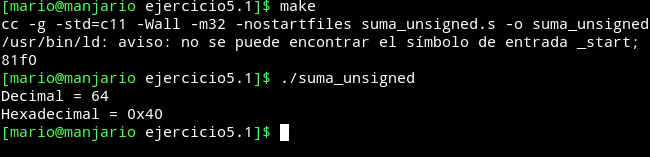
\includegraphics[scale=0.8]{ejercicio5.1/capturas/ej5-1.png} 
	\caption{Ejecución del programa "suma" SIN signo.} 
	\label{fig:figura1}
\end{figure}

\newpage

\section{Ejercicio 5.2: Suma CON signo en 32 bits}

\lstinputlisting{ejercicio5.2/suma_signo.s}

\begin{figure}[H] %con el [H] le obligamos a situar aquí la figura
	\centering
	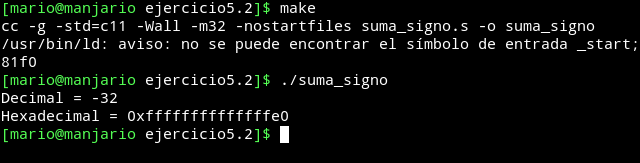
\includegraphics[scale=0.8]{ejercicio5.2/capturas/ej5-2.png}  
	\caption{Ejecución del programa suma CON signo.} 
	\label{fig:figura2}
\end{figure}

\newpage

\section{Ejercicio 5.3: Media CON signo en 32 bits}

\lstinputlisting{ejercicio5.3/media.s}

\begin{figure}[H] %con el [H] le obligamos a situar aquí la figura
	\centering
	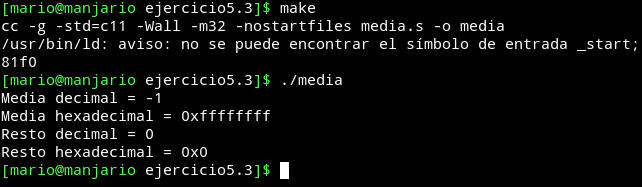
\includegraphics[scale=0.8]{ejercicio5.3/capturas/ej5-3.png}  
	\caption{Ejecución del programa media con signo.} 
	\label{fig:figura3}
\end{figure}

\newpage

\section{Preguntas de Auto-comprobación}
\subsection{Sesión de depuración saludo.s}
\begin{enumerate}
	\item \textbf{\textit{¿Qué contiene EDX tras ejecutar mov longsaludo, \%edx?
		 ¿Para qué necesitamos esa instrucción, o ese valor? Responder no sólo el valor concreto (en decimal y hex) sino también el significado del mismo (¿de dónde sale?). Comprobar que se corresponden los valores hexadecimal y decimal mostrados en la ventana Status‐>Registers.}}
	 
	 EDX, tras ejecutar \textbf{mov longsaludo}, contiene el valor 28 (hexadecimal 0x1C) como puede apreciarse en la Figura \ref{fig:figura4}
	 \begin{figure}[H] %con el [H] le obligamos a situar aquí la figura
	 	\centering
	 	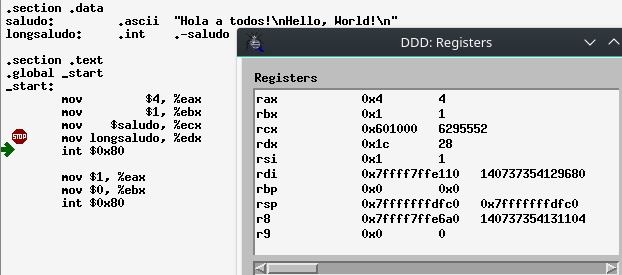
\includegraphics[scale=0.8]{capturas/saludo1.png}  
	 	\caption{Depuración de saludo.s} 
	 	\label{fig:figura4}
	 \end{figure}
	 EDX contiene este valor porque al alojarle el valor de la variable \textbf{longsaludo} que es el contador de posiciones de saludo: el número de bytes que ocupará. Es por ello que se necesite el uso de este valor ya que por medio ahora de esta instrucción se podrá indicar la que se escribirán 28 bytes.
	 
	\item \textbf{\textit{¿Qué contiene ECX tras ejecutar mov \$saludo, \%ecx? Indicar el valor en hexadecimal, y el significado del mismo.}}
	
	Como muestra la Figura \ref{fig:figura4}, ECX contiene el valor hexadecimal 0x601000. Este valor define la dirección en memoria del contenido de la cadena \textbf{saludo}.
	
	\item \textbf{\textit{¿Qué sucede si se elimina el símbolo de dato inmediato (\$) de la instrucción anterior? (mov saludo, \%ecx). Realizar la modificación, indicar el contenido de ECX en hexadecimal, explicar por qué no es lo mismo en ambos casos. Concretar de dónde viene el nuevo valor (obtenido sin usar \$).}}
	
	Si se elimina el símbolo de dato inmediato \$ de la instrucción  \textbf{mov \$saludo, \%ecx} en vez de mover la dirección de memoria de \textbf{saludo} al registro \textbf{ecx}, será el contenido de \textbf{saludo} el que se guarde en dicho registro. 
	
	\begin{figure}[H] %con el [H] le obligamos a situar aquí la figura
		\centering
		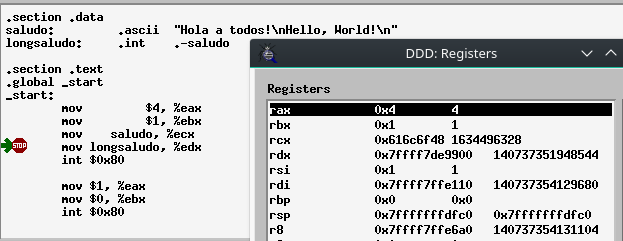
\includegraphics[scale=0.8]{capturas/saludo3.png}  
		\caption{Depuración de saludo.s} 
		\label{fig:figura5}
	\end{figure}
	
	Como se observa en la Figura \ref{fig:figura5}, el valor de \textbf{ECX} ahora es \textbf{0x616c6f48}, que es la representación en hexadecimal de la cadena de texto almacenada en \textbf{saludo}.
	
	\item \textbf{\textit{¿Cuántas posiciones de memoria ocupa la instrucción mov \$1, \%ebx? ¿Cómo se ha obtenido esa información? Indicar las posiciones concretas en hexadecimal.}}
	
	La instrucción mov \$1, \%ebx ocupa cinco posiciones de memoria.
	\begin{figure}[H] %con el [H] le obligamos a situar aquí la figura
		\centering
		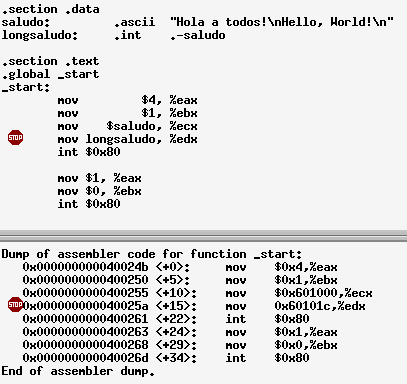
\includegraphics[scale=0.8]{capturas/saludo6.png}  
		\caption{Desensamblado de saludo.s} 
		\label{fig:figura6}
	\end{figure}
	
	Como se puede observar en la Figura \ref{fig:figura6} su posición se encuentra desde la dirección 0x0400250 hasta la 0x0400255. Esta información se obtiene desde la opción \textbf{"View -> Machine Code Window"} de \textbf{ddd}.
	
	\item \textbf{\textit{¿Qué sucede si se elimina del programa la primera instrucción int 0x80? ¿Y si se elimina la segunda? Razonar las respuestas}}
	
	Si se elimina la primera instrucción \textbf{int 0x80} el programa finaliza aparentemente sin errores, sin embargo no se imprimen los mensajes por pantalla.	
	Este hecho se produce porque con la instrucción \textbf{mov \$4, \%eax} se realiza una llamada a \textbf{write} (encargado de imprimir mensajes en pantalla). Ésta se pierde con la instrucción siguiente \textbf{mov \$1, \%eax}.
		
	Si eliminamos la segunda instrucción \textbf{int 0x80}, en esta ocasión sí que se producen errores en la finalización de la ejecución del programa, concretamente un fallo de segmentación. 	
	Este hecho se produce porque con la instrucción \textbf{mov \$1, \%eax} se realiza una llamada a \textbf{exit} (encargado de finalizar la ejecución de un programa) Al no producirse esta llamada el programa no sabe cómo establecer el final de la ejecución y produce un fallo de segmentación.
	
	\item \textbf{\textit{¿Cuál es el número de la llamada al sistema READ (en kernel Linux 32bits)? ¿De dónde se ha obtenido esa información?}}
	
	El número de la llamada al sistema READ (en kernel Linux 32bits) es el 3.	
	\begin{figure}[H] %con el [H] le obligamos a situar aquí la figura
		\centering
		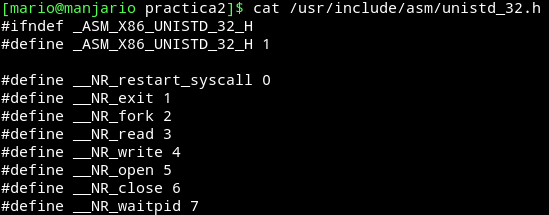
\includegraphics[scale=0.8]{capturas/saludo8.png}  
		\caption{Llamadas al sistema} 
		\label{fig:figura8}
	\end{figure}
	Esta información puede obtenerse, por ejemplo, en el archivo \textbf{unistd\_32.h} del directorio \textbf{/usr/include/asm/} como muestra la Figura \ref{fig:figura8}
		 
\end{enumerate}

\subsection{Sesión de depuración suma.s}
\begin{enumerate}
	\item \textbf{\textit{¿Qué dirección se le ha asignado a la etiqueta suma? ¿Y a bucle? ¿Cómo se ha obtenido esa información?}}
	
	La dirección que se le ha asignado a la etiqueta \textbf{suma} es \textbf{0x804822a}(Figura \ref{fig:suma3}) y \textbf{0x8048235} a \textbf{bucle} (Figura \ref{fig:suma3-2}).
	
	\begin{figure}[H] %con el [H] le obligamos a situar aquí la figura
		\centering
		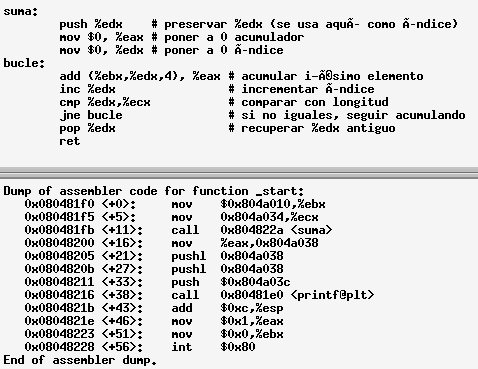
\includegraphics[scale=0.8]{capturas/suma3.png}  
		\caption{Desesamblado de suma.s} 
		\label{fig:suma3}
	\end{figure}
	\begin{figure}[H] %con el [H] le obligamos a situar aquí la figura
		\centering
		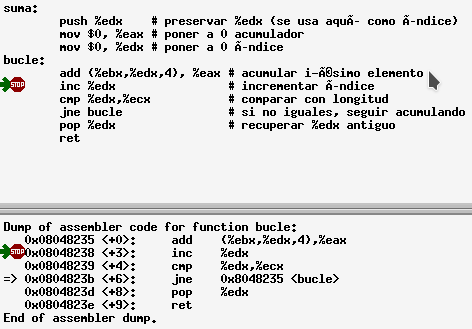
\includegraphics[scale=0.8]{capturas/suma3-2.png}  
		\caption{Desesamblado de suma.s} 
		\label{fig:suma3-2}
	\end{figure}

	Esta información se ha obtenido desde la opción \textbf{"View -> Machine Code Window"} de \textbf{ddd}.
	
	\item \textbf{\textit{¿Para qué usa el procesador los registros EIP y ESP?}}
	
	El procesador usa el registro \textbf{EIP} como puntero a la siguiente dirección de memoria que va a ejecutar y el registro \textbf{ESP} lo usa como puntero al inicio de la pila del programa.
	
	\item \textbf{\textit{¿Qué registros modifica la instrucción CALL? Explicar por qué necesita CALL modificar esos registros.}}
	
	La instrucción \textbf{CALL} modifica los registros \textbf{EAX} (al funcionar como acumulador debe ir modificándose tras cambiar el resultado de la suma), \textbf{EDX} (se modifica porque es un índice que muestra la siguiente dirección de memoria a leer), \textbf{ESP} (es modificado ya que en él se alojará la dirección de retorno al pasar por RET) y \textbf{EIP} y EIP (se altera porque en él se encuentra la dirección de la instrucción siguiente que se va a ejecutar).
	
	\item \textbf{\textit{¿Qué registros modifica la instrucción RET? Explicar por qué necesita RET modificar esos registros.}}
	
	La instrucción \textbf{RET} modifica los registros \textbf{ESP} y \textbf{EIP} ya que éstos actúan como punteros y deben cambiar su contenido para que el programa pueda seguir con su ejecución desde el punto en el que se encontraba antes de llamar a la subrutina.
	
	\item \textbf{\textit{¿Qué ocurriría si se eliminara la instrucción RET? Razonar la respuesta. Comprobarlo usando ddd.}}
	
	Si se eliminara la instrucción \textbf{RET} sería imposible devolver la ejecución al programa principal desde el que se llamó a la subrutina. Esto daría lugar a un error en la ejecución del programa provocando un fallo de segmentación.
\end{enumerate}

\end{document}
